\documentclass{article}

\usepackage[dvipsnames,svgnames,x11names]{xcolor}
\usepackage[preprint]{corl_2026}

\usepackage{amsmath, amssymb}
\usepackage{graphicx}
\usepackage{float}
\usepackage{booktabs}
\usepackage{caption}
\usepackage{subcaption}
\usepackage{algorithm}
\usepackage{algpseudocode}
\usepackage{tikz}
\usetikzlibrary{arrows.meta, positioning, calc}

\definecolor{cblue}{HTML}{4A90D9}
\definecolor{cgreen}{HTML}{5BAD72}
\definecolor{corange}{HTML}{E8863A}
\definecolor{cpurple}{HTML}{9B6BBE}
\definecolor{cgray}{HTML}{7F8C8D}

\title{LeWAM: A JEPA-based World Action Model}

\author{
  Eryk Halicki\\
  University of British Columbia, ETH Zurich\\
  \texttt{ehalicki@student.ubc.ca}\\
}

\begin{document}

\maketitle

\begin{abstract}
    World Action Models (WAMs) that jointly predict future video latents and decode actions from those predictions have recently shown strong zero-shot generalization across robot embodiments\cite{DreamZero}\cite{MimicVideo}.
However, existing WAMs rely on large-scale compute infrastructure that is inaccessible to most researchers.
We present \textbf{LeWAM}, a compact World Action Model designed to run on consumer hardware.
LeWAM combines a frozen-pretrained V-JEPA2 video encoder with a lightweight flow-matching Diffusion Transformer (DiT) that predicts future patch embeddings in latent space, and an Inverse Dynamics Model (IDM) that decodes action chunks from the predicted transitions.
The separation of video prediction and action decoding allows the DiT to be pretrained on unlabeled internet video, and the IDM to be finetuned independently on small robot datasets.
We apply Sketched Isotropic Gaussian Regularization (SIGReg)~\citep{LeJEPA,LeWorldModel} to stabilize JEPA training and train on the SmolVLA community dataset~\citep{SmolVLA}.
Despite operating at a fraction of the parameter count of prior WAMs, LeWAM achieves competitive performance on [TODO: benchmark], demonstrating that strong video-conditioned action prediction does not require server-scale compute.
\end{abstract}

\keywords{World Action Model, Robot Learning, Flow Matching, Efficient Inference, Video Prediction}

%===============================================================================

\section{Introduction}

World Action Models (WAMs) have recently emerged as a powerful paradigm for robot learning, jointly predicting future video and robot actions from a shared dynamics model.
By inheriting rich dynamics priors from internet-scale video pretraining, WAMs like DreamZero~\cite{DreamZero} and MimicVideo~\cite{MimicVideo} achieve remarkably data-efficient training and strong zero-shot generalization across embodiments, environments, and tasks.
However, these models rely on heavyweight pixel space and latent video diffusion backbones with billions of parameters, requiring server-scale compute (GB200, H100 GPUs) for both training and inference. This places them out of reach for smaller labs and the open-source robotics community, and makes them prohibitively difficult to deploy in real-world settings.

Thankfully, this reliance on pixel-space and latent video diffusion may be unnecessary.

DreamZero and MimicVideo both achieve negligible performance loss, or even performance gains, when only partially denoising future video frames, suggesting that fine-grained visual details contribute little to action prediction.
This observation is consistent with JEPA-style models~\cite{vjepa2_1, LeWorldModel, IJEPA}, which show that predicting in latent space is far more compute-efficient than pixel-space reconstruction while retaining the dynamics information relevant to downstream tasks, such as robotic control~\cite{LeWorldModel, vjepa2_1}.

% Although previous JEPA world models have been adapted for robotic manipulation \citep{LeWorldModel, vjepa2_1}, they require expensive inference-time planning and lack language conditioning, limiting their practical applicability. VLA-JEPA~\cite{VLAJEPA} addressed this with a joint world-action modeling objective built on V-JEPA2 latents, achieving promising results. However, their approach separates the latent world model and action head into distinct components, and relies on a computationally heavy VLM backbone. 

Separately, SmolVLA~\cite{SmolVLA} has demonstrated that competitive robot policies can be trained at small scale on consumer hardware, but to our knowledge, this accessibility has not yet been achieved for World-Action Models. 

To bridge this gap, we present \textbf{LeWAM}, a compact latent-space World-Action Model.

% LeWAM uses a distilled and frozen V-JEPA~2.1~\cite{vjepa2_1} encoder as its visual backbone, SmolVLM2~\cite{SmolVLM2, SmolVLA} for visually grounded language conditioning, and a flow-matching Diffusion Transformer (DiT) that jointly denoises future video latents and action trajectories in a single forward pass.

By operating entirely in latent space and sharing a single transformer across both prediction targets, LeWAM requires only 500M parameters, a fraction of the data and compute budget of prior WAMs, and trains and runs on a single consumer GPU.



 
 


%===============================================================================

\section{Related Work}

\subsection{World Action Models}
World-Action Models (WAMs) are models that combine world modelling and action prediction into a tightly coupled architecture. Some previous works have described their approach as using Video-Action Models~\cite{MimicVideo, UVAM}, Vision-Language-Action models with a world modelling objective\cite{VLAJEPA, won2025dual}, or Video-Language-Action models~\cite{GR-2}, however the category of World-Action models, as defined in \citet{DreamZero}, encapsulates all these approaches. The common point that ties them together is their utilization of a future state predicting objective alongside action prediction. Although the most common to date, video is just one world modelling modality; future work, including our proposed method, may utilize alternate predictive modalities, such as learned latent represenations, 3D pointclouds, tactile senses, auditory signals, or a multimodal combination of others.

World-Action Models present a distinct strength when compared to the more prevalent Vision-Language-Action Models (of the non-world modelling variety); the ability to learn from diverse data sources. Most VLA architectures are constrained by the prohibitive cost of collecting successful expert demonstrations in a large variety of settings. WAMs on the other hand, are more natively able to learn from diverse environmental interaction data, and have been shown to improve multi-task performance, sample efficiency, and generalization to novel scenes and objects~\cite{DreamZero, MimicVideo, UWM, TRIWAM, CosmosPolicy}.

These strengths come at a cost, since many current World-Action models rely on large-scale video diffusion models for their dynamics priors, often being prohibitively expensive to train and deploy in real time or on edge hardware~\cite{DreamZero}. 

%Although our proposed method forgoes these video generation priors, we build on the strong latent representations of V-JEPA2 to reduce training and inference cost, while aiming to retain the sample efficiency and generalization benefits characteristic of WAMs.

\subsection{Vision Language Action Models}
Foundational to the recent successes in robot learning, Vision Language Action models have paved the way for generalizable and robust systems that can learn dozens or even hundreds of behaviours~\cite{pi0.5, GrootN1, geminirobotics, Octo} within a single policy. VLAs have shown great promise, but suffer from the previously mentioned limitations of data inefficiency, requiring hundreds to thousands of hours of largely repeated demonstrations to effectively generalize\cite{pi0.5, geminirobotics}. Co-training VLAs on non-robot web data improves performance in some cases~\cite{pi0.5}, but its effect is not nearly as pronouced as in WAMs.

Many leading VLAs deal with the same high computational costs as WAMs. This has motivated works like \citet{SmolVLA} and \citet{TinyVLA} to design compact VLA architectures, allowing for more accessible training and deployment, while maintaining competetive performance with leading models. To the best of our knowledge, such small scale approaches have yet to be replicated in WAMs, motivating our own approach. 

% https://arxiv.org/pdf/2507.05331

\subsection{Joint Embedding Prediction (JEPA)}
Joint Embedding Predictive Architectures, or JEPAs, are a series of world modelling architectures that prioritize semantic understanding over visual fidelity, improving efficiency over generative approaches, while acheiving comparable or superior performance on downstream tasks~\cite{vjepa2, vjepa2_1, IJEPA}. Characteristically, they differ from generative approaches like VAEs or diffusion models by exclusively operating in latent space. 

Recent works using video JEPA models have shown promising results in robotic control tasks~\cite{vjepa2, vjepa2_1, LeWorldModel}. Rather than an action-generative approach ($p(z_{i+1}, a_{i+1}| z_i)$), most JEPA works have adopted an action-conditioned formulation ($p(z_{i+1} | z_i, a_{i+1})$). This approach does have some distinct strengths (e.g. controllability), but it requires expensive inference-time planning and lacks language conditioning, limiting its practical applicability. Our proposed method instead aims to inherit the semantic and dynamic understanding properties of video JEPA models while adopting the more common action generative approach used throughout VLAs and WAMs.

\subsection{Latent World-Action Models}

%Many video and image generation models have adopted a latent-space diffusion approach to improve efficiency over pixel space diffusion~\cite{wan, latentdiffusion, CosmosPredict2.5}. Consequentially, many WAMs that build off of these generative models also adopt a latent diffusion formulation~\cite{DreamZero, MimicVideo}. However, there is a fundamental mismatch between the requirements of video generation models and WAMs, namely visual fidelity.

Although improved video generation quality has been shown to directly improve action prediction performance~\cite{DreamZero, MimicVideo}, we argue that the reliance on latents produced by Video VAEs introduces unnessecary bulk into WAMs, since they encode fine grained visual details (eg. lighting, fine grained textures) that may not be relevant to robotic manipulation tasks.

Similarly, VLA-JEPA~\cite{VLAJEPA} aims to mitigate this reliance on pixel-space VAEs by adopting a V-JEPA2 encoder alongside a generative world-action modelling objective, with promising results. However, the work mainly focuses on latent-action pretraining, and seperates their autoregressive transformer latent world model and flow matching action head. Furthermore, VLA-JEPA adopts a signficantly larger VLM backbone, V-JEPA2 encoder, world model, and action head than we do. Consequentially, their model utilizes the same amount, if not more parameters than leading VLAs\cite{pi0.5}. [TODO: calculate exact parameter count of VLA-JEPA since they dont share it]

In contrast to \citet{VLAJEPA}, our proposed method does not focus on latent-action pretraining, and unifies the world model and action head into a single DiT. We also target a much smaller scale regime, similar to \citet{SmolVLA} and \citet{TinyVLA}


%===============================================================================

\section{Method}

\subsection{Overview}

LeWAM jointly predicts future video latents and robot actions using a single conditional flow-matching Diffusion Transformer~\cite{DiT, FlowMatching, esser2024scaling}, following the joint video-action denoising approach of ~\citet{DreamZero}, \citet{UWM}, and \citet{CosmosPolicy}. Rather than the VAE latents used by most other WAMs, our proposed method denoises video latents from a JEPA video encoder.

The model processes a sequence of three token groups: (1) \textbf{context video tokens} (clean), (2) \textbf{future video tokens} (noisy), and (3) \textbf{action tokens} (noisy), with a block-causal attention mask that enforces temporal ordering.
A frozen V-JEPA~2.1 encoder~\cite{vjepa2_1} provides the video representation used for both context and future ground truth. Additionally, a frozen SmolVLM2~\cite{SmolVLM2, SmolVLA} and an unfrozen state encoder provide visually-grounded language and state conditioning via cross-attention~\cite{GenTron}.

Figure~\ref{fig:arch} illustrates the full architecture.

[TODO: add model parameters to appendix (depth, model dimensions, action loss weight used in training, etc.)]

%---------------------------------------

\subsection{Video Encoder}

We use V-JEPA~2.1~\citep{vjepa2_1} ViT-B as our visual encoder, initialized from pretrained weights and frozen during training. The ViT-B variant was distilled from the main ViT-G model, reducing it to only 80 million parameters. 

All camera views are concatenated horizontally, then divided into spatial patches of size $16 \times 16$ and grouped into tubelets of temporal size 2, halving the temporal token count.
We use a crop size of $256 \times 256$ per input image in practice, producing a $16 \times 16$ token grid per camera per frame, although the use of 3D-RoPE interpolation~\cite{ThreeDRoPE} in both VJEPA2 and our DiT allows for this value to be changed at inference-time.

Given $C$ context frames and horizon $H$, the encoder produces context latents $\mathbf{z}_{0:C} \in \mathbb{R}^{H_p W_p \times D_{\text{enc}}}$ and future targets $\mathbf{z}_{C:H} \in \mathbb{R}^{H_p W_p \times D_{\text{enc}}}$, where $D_{\text{enc}} = 768$.

%---------------------------------------

\subsection{Visually Grounded Language Conditioning}

We use SmolVLM2-256M~\cite{SmolVLM2, SmolVLA} as our language encoder for its compact size and video pretraining, although the 500M variant can be used as a drop in replacement like in \citet{SmolVLA}. The VLM's vision encoder and connector are used to encode image or video context, which is prepended to the language token sequence before passing through the first $N$ language model layers. Similar to SmolVLA, instead of using only the hidden state after layer $N$, we store every intermediate hidden state $h_{i \in [1, N]}$, and have DiT block $i$ cross attend to the hidden state $h_i$.

During training, language conditioning is dropped with probability $p_{\text{drop}} = 0.15$ to enable classifier-free guidance at inference time~\cite{DreamZero}.

%---------------------------------------

\subsection{Joint Flow-Matching DiT}

Unlike some WAMs that use separate models for video and action prediction~\cite{MimicVideo, VLAJEPA, TRIWAM}, we adopt the joint denoising formulation of ~\citet{DreamZero}, \citet{UWM}, and \citet{CosmosPolicy},  predicting both future video latents and actions jointly in a single DiT. The input sequence is constructed by concatenating the context, future, and action tokens. Noise is added in the native action and encoder spaces ($D_{\text{action}}$ and $D_{\text{enc}}$) before projection to $D$ via separate linear layers.

\paragraph{DiT Block Structure.}
Each transformer layer consists of: (1) \textbf{block-causal self-attention} over the full token sequence with 3D-RoPE positional encoding~\cite{ThreeDRoPE, DreamZero, vjepa2_1} (see Appendix~\ref{attn_structure}), where video tokens receive $(t, h, w)$ position IDs and action tokens receive $(t, 0, 0)$; (2) \textbf{cross-attention} to proprioceptive state (encoded via a two-layer MLP) and language tokens from SmolVLM2; and (3) an \textbf{MLP} feedforward block. All sub-layers use adaLN-Zero~\citep{DiT} conditioning on the timestep embedding $\tau(t)$, with weights initialized to zero for stable early training.

\paragraph{Flow Matching Objective.}

Given a training sample with context latents $\mathbf{z}_{0:C}$, future targets $\mathbf{z}_{C:H}$, target actions $\mathbf{a}_{C:H}$, state $\mathbf{s}_{C-1}$, image $\mathbf{I}_{C-1}$, and language tokens $\mathbf{l}_{C-1}$, we sample noise $\boldsymbol{\epsilon}_z \sim \mathcal{N}(0, I)$, $\boldsymbol{\epsilon}_a \sim \mathcal{N}(0, I)$, and a shared timestep $t \sim \mathcal{U}[0, 1]$.
The noisy inputs are constructed via linear interpolation:
\begin{equation}
    \mathbf{z}_t = (1 - t)\,\boldsymbol{\epsilon}_z + t\,\mathbf{z}_{C:H}, \qquad \mathbf{a}_t = (1 - t)\,\boldsymbol{\epsilon}_a + t\,\mathbf{a}_{C:H}.
\end{equation}

The model predicts velocity fields $\hat{\mathbf{v}}_z, \hat{\mathbf{v}}_a = f_\theta(\mathbf{z}_t, \mathbf{a}_t, \mathbf{z}_{0:C}, t, \mathbf{s}_{C-1}, \mathbf{I}_{C-1}, \mathbf{l}_{C-1})$, and the flow matching loss is:
\begin{equation}
    \mathcal{L}_{\text{flow}} = \left\| \hat{\mathbf{v}}_z - (\mathbf{z}_{C:H} - \boldsymbol{\epsilon}_z) \right\|^2 + \lambda_a \left\| \hat{\mathbf{v}}_a - (\mathbf{a}_{C:H} - \boldsymbol{\epsilon}_a) \right\|^2,
\end{equation}
where $\lambda_a$ balances the video and action losses.

\paragraph{Inference}

At inference time, we sample initial noise for both video latents and actions and integrate the learned velocity field from $t = 0$ to $t = 1$ using Euler integration:
\begin{equation}
    \hat{\mathbf{z}}_{t+\Delta t} = \hat{\mathbf{z}}_t + \hat{\mathbf{v}}_z \cdot \Delta t, \qquad \hat{\mathbf{a}}_{t+\Delta t} = \hat{\mathbf{a}}_t + \hat{\mathbf{v}}_a \cdot \Delta t.
\end{equation}

The predicted actions are optionally smoothed using a Savitzky-Golay filter to remove high frequency noise left over from the denoising process~\cite{DreamZero}.

\paragraph{Action normalization.}
Actions and proprioceptive state are normalized using precomputed dataset statistics. Values are clipped to the 1st/99th percentiles and z-scored, preventing outliers from distorting the learning signal.

%---------------------------------------

\subsection{Training}

\begin{figure}[h]
    \centering
    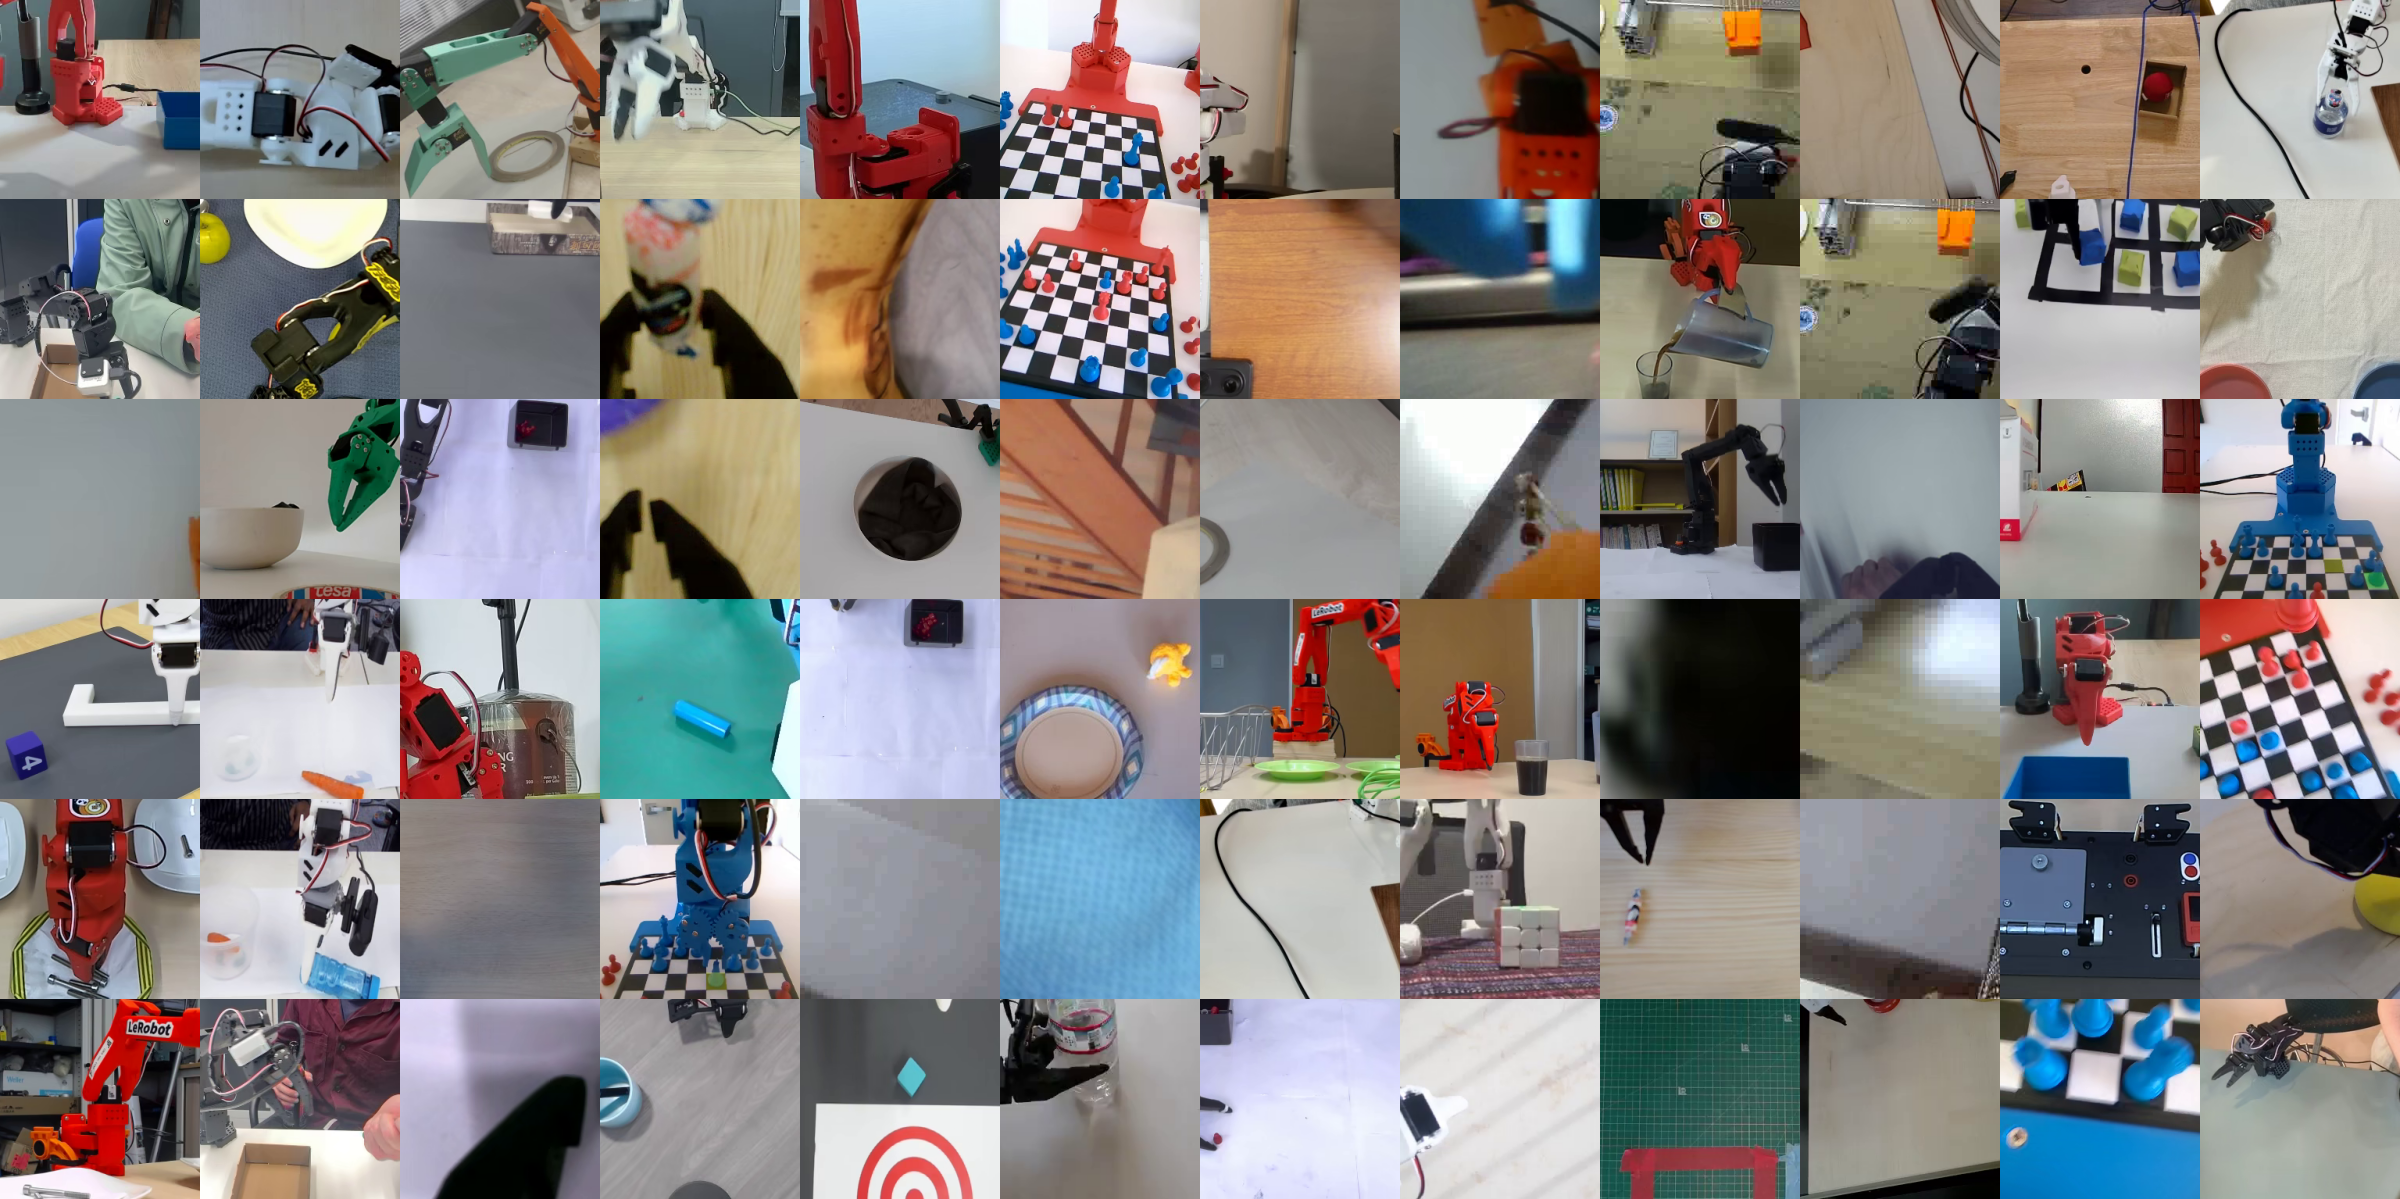
\includegraphics[width=\textwidth]{figures/generated/dataset_grid.png}
    \caption{A sample of episodes from the HuggingFaceVLA community dataset used for pretraining in SmolVLA\cite{SmolVLA} and our proposed method.}
    \label{fig:dataset}
\end{figure}

\paragraph{Robot pretraining data.}
We train on the open-source HuggingFaceVLA community dataset utilized in \citet{SmolVLA} (HuggingFace: \texttt{HuggingFaceVLA/community\_dataset\_v2}). The dataset is a collection of community-contributed robot manipulation demonstrations from the SO-101 and SO-100 low-cost arms, spanning 60 hours of in-the-wild data collected using the LeRobot framework~\cite{LeRobot}.

Most of the data preprocessing follows ~\citet{SmolVLA}, however new demonstrations were added in the second iteration of the dataset, prompting additional data preprocessing which was not done in the original SmolVLA project. Some added datasets did not match the SO-101/100 embodiments, and a handful of demonstrations had undescriptive task labels; such episodes were either manually deleted or relabeled. 

Additionally, the original dataset was published using the LeRobotDataset v2.1 format, which is deprecated. To better support modern tooling, we converted the entire to dataset to LeRobotDataset v3.0 and published it on HuggingFace (HuggingFace: \texttt{ehalicki/LeWAM\_community\_dataset})

\paragraph{Finetuning data.}
For our fine tuning experiments we collected [TODO: currently projecting ~200] demonstrations across 4 tasks using the SO-101 arm, similar to \citet{SmolVLA}. 

[TODO describe the tasks (pick and place, sorting, stacking)]

\paragraph{Training schedule}

[TODO: fill in once pre training and fine tuning schedules are finalized]

%---------------------------------------

[TODO: add a python pseudocode section like LeWorldModel]


%===============================================================================

\section{Experiments}

[TODO: the final set of experiments is still being decided; the descriptions below outline candidate directions]

\subsection{Real World Tasks}

We plan to evaluate on the same real world manipulation tasks as SmolVLA, with SmolVLA, ACT, and a diffusion policy as baselines. We also want to test zero-shot generalization in the style of DreamZero on tasks not seen during fine tuning.

\subsection{LIBERO}

We plan to report results on LIBERO as a standardized benchmark, for more direct comparison against prior work.

\subsection{Ablations}

\subsubsection{World Modelling Objective}

Does the video latent prediction objective help, and when? We want to measure its effect in the single task and multi task regimes, with and without pretraining.

\subsubsection{JEPA vs Video VAE vs Pixel Space}

Does a V-JEPA2 backbone actually help, or would a similarly sized video VAE work just as well? Candidate drop-in replacements include the CogVideoX VAE, OmniTokenizer-VAE, and Cosmos-Tokenizer-CV. We also want to check whether pixel space diffusion is competitive at this scale.

\subsubsection{Pretraining}

Does pretraining on community data improve downstream task performance compared to training from scratch?

\subsubsection{Diverse Data}

Does fine tuning on diverse tasks lead to cross task generalization relative to single task fine tuning?

\subsection{Cross-Embodiment Transfer}

Can the model learn out of distribution tasks from video-only data on different embodiments, including egocentric human video?

\subsection{Classifier Free Guidance}

DreamZero uses CFG at inference. Does it help here, and does it change how the policy behaves?

\subsection{Continual Learning}

Can the video prediction component keep improving from the policy's own rollouts?


%===============================================================================

\input{sections/results}

%===============================================================================

\section{Discussion}

[TODO: highly dependant on experiment results]


%===============================================================================

\section{Conclusion}

[TODO: dependant on experiment results]


\acknowledgments{}

\bibliography{ref}

\appendix
\section{Appendix}

\end{document}
